\documentclass[tikz,border=4pt]{standalone}
% Shared style for every figure and for the deck: one accent, one
% highlight, thin lines, rounded nodes, nothing decorative.
\usepackage[T1]{fontenc}
\usepackage{lmodern}
\renewcommand{\familydefault}{\sfdefault}
\usepackage{tikz}
\usetikzlibrary{arrows.meta,positioning,calc,shapes.misc,fit,backgrounds,decorations.pathreplacing}
\definecolor{ink}{RGB}{40,40,40}
\definecolor{soft}{RGB}{150,150,150}
\definecolor{faint}{RGB}{225,225,225}
\definecolor{accent}{RGB}{0,95,115}
\definecolor{accentlight}{RGB}{214,232,236}
\definecolor{warn}{RGB}{196,84,40}
\definecolor{warnlight}{RGB}{247,226,216}
\tikzset{
  every picture/.style={color=ink, line width=0.5pt, font=\small},
  node distance=12mm and 18mm,
  box/.style={draw=ink, rounded corners=2pt, fill=white, inner sep=5pt, minimum height=7mm, align=center},
  maker/.style={box, minimum width=18mm},
  cat/.style={box, inner sep=3.5pt, minimum height=6mm},
  root/.style={box, fill=accentlight, draw=accent},
  bad/.style={box, fill=warnlight, draw=warn},
  ghost/.style={box, draw=soft, text=soft, dashed},
  flow/.style={-{Stealth[length=4pt,width=3.5pt]}, line width=0.5pt},
  sub/.style={-{Stealth[length=4pt,width=3.5pt]}, line width=0.5pt, color=soft},
  strong/.style={flow, color=accent, line width=0.8pt},
  wrong/.style={flow, color=warn},
  lbl/.style={font=\footnotesize, text=ink, inner sep=1.5pt, fill=white},
  note/.style={font=\footnotesize, text=soft, align=center},
  rate/.style={font=\footnotesize, text=accent, inner sep=1pt, fill=white},
}

\usepackage{amsmath}
\usepackage{pgfplots}
\pgfplotsset{compat=1.17}

\begin{document}
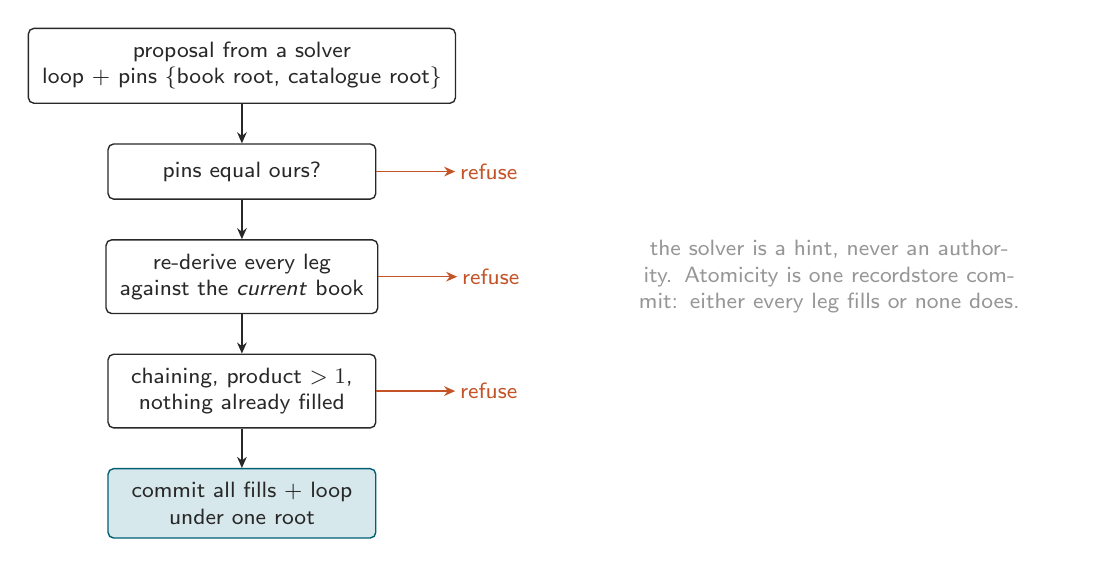
\begin{tikzpicture}[stp/.style={box, minimum width=34mm, align=center, font=\footnotesize}]
  \node[stp] (p) {proposal from a solver\\ loop + pins \{book root, catalogue root\}};
  \node[stp, below=5mm of p] (s0) {pins equal ours?};
  \node[stp, below=5mm of s0] (s1) {re-derive every leg\\ against the \emph{current} book};
  \node[stp, below=5mm of s1] (s2) {chaining, product $>1$,\\ nothing already filled};
  \node[stp, root, below=5mm of s2] (s3) {commit all fills + loop\\ under one root};
  \draw[flow] (p) -- (s0); \draw[flow] (s0) -- (s1); \draw[flow] (s1) -- (s2); \draw[flow] (s2) -- (s3);
  \foreach \n in {s0,s1,s2} { \draw[wrong] (\n.east) -- ++(10mm,0) node[lbl, right, text=warn] {refuse}; }
  \node[note, text width=60mm, right=26mm of s1] {the solver is a hint, never an authority. Atomicity is one recordstore commit: either every leg fills or none does.};
\end{tikzpicture}
\end{document}
